\documentclass{article}
\setlength{\parskip}{5pt} % esp. entre parrafos
\setlength{\parindent}{0pt} % esp. al inicio de un parrafo
\usepackage{listings} % listings
\usepackage{color} %colores
\usepackage{amsmath} % mates
\usepackage[sort&compress,numbers]{natbib} % referencias
\usepackage{url} % que las URLs se vean lindos
\usepackage[top=15mm,left=20mm,right=20mm,bottom=25mm]{geometry} % margenes 
\usepackage{hyperref} % ligas de URLs
\usepackage{graphicx} % poner figuras
\usepackage[spanish]{babel} % otros idiomas
\usepackage{caption}
\usepackage{subcaption}

\author{Claudia Lizeth Hern\'andez Ram\'irez} % author
\title{Homework 12 - Red Neuronal} % titulo
\date{\today}

\definecolor{myfucsia}{rgb}{1, 0.078, 0.576}
\definecolor{mygray}{rgb}{0.752, 0.752, 0.752}
\definecolor{mypurple}{rgb}{0.580, 0, 0.827}
\lstset{ 
  backgroundcolor=\color{mygray},
  commentstyle=\color{myfucsia},
  keywordstyle=\color{mypurple}, 
  numberstyle=\tiny\color{myfucsia}
  stringstyle=\color{mypurple}, 
  breaklines=true,
}


\begin{document} % inicia contenido

\maketitle % cabecera



% INTRODUCCIOOOOOOOOOOOON
\section{Introducci\'{o}n}\label{intro} % seccion y etiqueta
Estudia de manera sistem\'atica el desempeño de la red neuronal en t\'erminos de su F-score para los diez d\'igitos en funci\'on de las tres probabilidades asignadas a la generaci\'on de los d\'igitos (ngb), variando a las tres en un experimento factorial adecuado.


% DESARROLLOOOOOOOOOOOO
\section{Desarrollo}\label{desarrollo} % Desarrollo de la tarea
Trabaj\'e con el codigo visto en clase \citep{CBase}, al cual se le agregaron algunas modificaciones para cumplir con el objetivo de la tarea. Antes que otra cosa, investigu\'e sobre el \texttt{F-Score}, y me percat\'e de que hay tres f\'ormulas para obtenerlo \citep{FScore1} \citep{FScore2}.

\begin{equation}
\label{eq:Precision}
Precision = \dfrac {True Positives}{True Positives + False Negatives}
\end{equation}

\begin{equation}
\label{eq:Recall}
Recall = \dfrac {True Positives}{True Positives + False Positives}
\end{equation}

\begin{equation}
\label{eq:FScore}
F-Score = \dfrac {2 * Precision * Recall}{Precision + Recall}
\end{equation}

Con esta informaci\'on adecu\'e las ecuaciones \ref{eq:Precision}, \ref{eq:Recall} y \ref{eq:FScore} para mi c\'odigo.


\begin{lstlisting}[language=R, caption= Segmento de c\'odigo ecuaci\'on F-Score.]
    precision = diag(contadores) / colSums(contadores[,1:10])
        recall <- diag(contadores) / rowSums(contadores)
        fscore <- (2 * precision * recall) / (precision + recall)
\end{lstlisting}

Tambi\'en trabaj\'e con varios ciclos \texttt{FOR} con los cuales variaba la probabilidad con la que mis cuadros \texttt{negro, gris y blanco} aparecer\'ian. Trabaj\'e con 6 replicas.

\begin{table}[ht]
    \centering
    \caption{Probabilidades por grupo.} 
    \begin{tabular}{|r|r|r|r|}
    \hline
     & Negro & Gris & Blanco  \\
    \hline
    1 & 0.8 & 0.5 & 0.002 \\
    \hline
    2 & 0.9 & 0.8 & 0.01 \\
    \hline
    3 & 0.995 & 0.92 & 0.5\\
    \hline
\end{tabular}
    \label{cuadro 1}
\end{table}


\begin{lstlisting}[language=R, caption= Segmento de c\'odigo ciclos \texttt{FOR}.]
replica = 1:6 #Replicaaas
negro<-c(0.8, 0.9, 0.995) #probabilidad encender cuadritos negros
gris<-c(0.5, 0.8, 0.92) #probabilidad encender cuadritos grises
blanco<-c(0.002, 0.01, 0.5) #probabilidad encender cuadritos blancos

for(ne in negro){
  for(gr in gris){
    for(bl in blanco){
      for(reply in replica){
        modelos <- read.csv("digits.txt", sep=" ",
                            header=FALSE, 
                            stringsAsFactors=F)
        modelos[modelos=='n'] <- ne
        modelos[modelos=='g'] <- gr
        modelos[modelos=='b'] <- bl
\end{lstlisting}

Toda esta informaci\'on la almacen\'e en una \texttt{Data Frame}.
\begin{lstlisting}[language=R, caption= Segmento de c\'odigo Data Frame.]
eale = c(reply, ne, gr, bl, fscore)
        datos = rbind(datos, eale)
        names(datos) = c("Replica", "Negro", "Gris", "Blanco",
                         "0", "1", "2", "3", "4", "5", "6", "7", "8", "9")
\end{lstlisting}

Posteriormente realic\'e la gr\'afica \ref{Figura 1} .
\begin{lstlisting}[language=R, caption= Segmento de c\'odigo Gr\'afica.]
gr = ggplot(dat.m, aes(x= combo, y= value, fill= combo)) +
      geom_violin(fill = "#D29BFD")
  gr + geom_boxplot(fill = colorRampPalette(c("#FF1694", "#FC46AA","#F25278", 
                                             "#FC4C4E", "#FE7D6A", "#FC9483",
                                            "#FC94AF", "#F79AC0", "#FA86C4"))(27), 
                      width = 0.3, lwd = 0.3) +
      theme(axis.text.x = element_text(angle = 90, vjust = 0.5, hjust=1),
            panel.background = element_rect(fill = "#CDCDCD")) +
      labs(x="combinacion de probabilidades", y= "f-score")
\end{lstlisting}

\begin{figure}[htb!] % figura
    \centering
    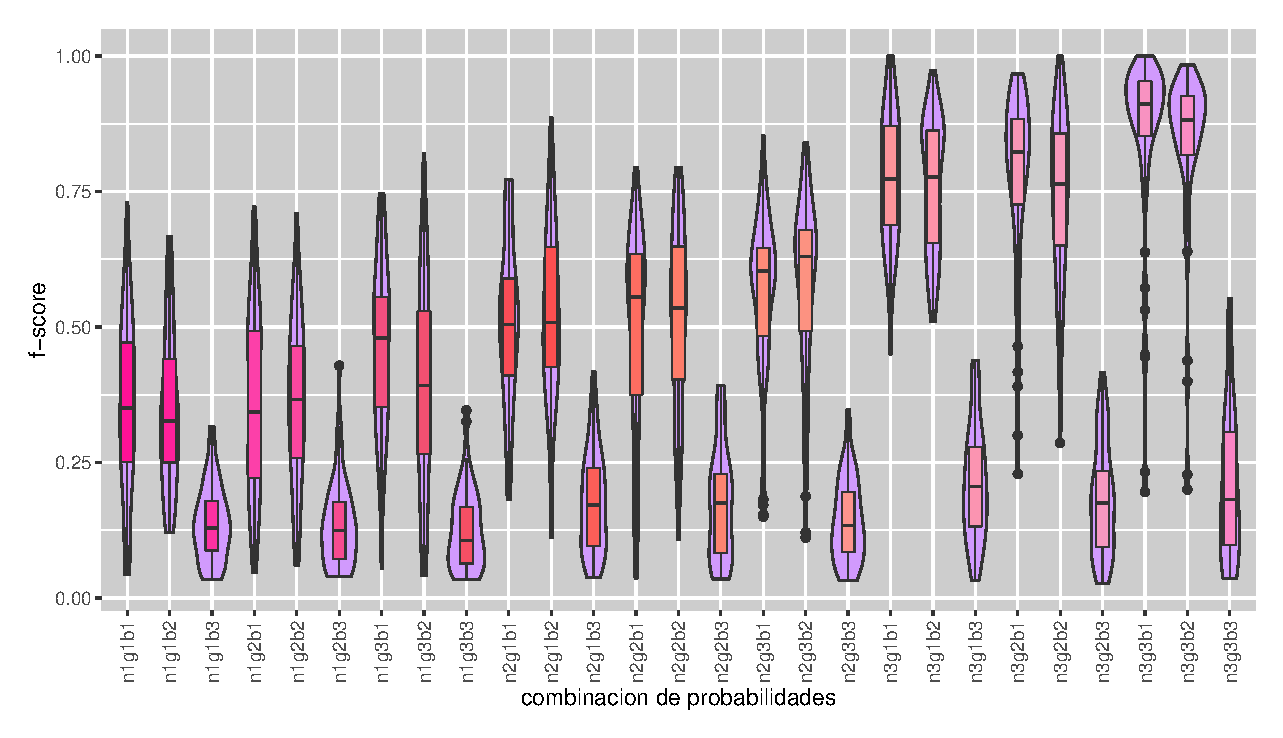
\includegraphics[width=150mm]{DLD.eps} % archivo
    \caption{F-Score vs Probabilidad.}
    \label{Figura 1}
\end{figure}


\section{Estad\'istica}

\begin{lstlisting}[language=R, caption= Segmento de c\'odigo Pruebas Estad\'isticas .]
    #Estad\'isitica - 
    #con p menor a 0.05 se rechaza hipotesis nula H0
    #H0: los datos proceden de una distribuci\'on normal
    #H1: los datos no proceden de una distribuci\'on normal
    tapply(dat.m$value, dat.m$combo, shapiro.test)
    
      
    ala = dat.m%>%
      group_by(combo) %>%
      summarise(
        cantidad_de_participantes = n(),
        promedio = mean(value, na.rm = TRUE),
        desviacion_estandar = sd(value, na.rm = TRUE),
        varianza = sd(value, na.rm = TRUE)^2,
        mediana = median(value, na.rm = TRUE),
        rango_intercuartil =  IQR(value, na.rm = TRUE)
      )
    
    kruskal.test(value ~ combo, data = dat.m)
\end{lstlisting}

\begin{table}[ht]
    \centering
    \caption{Resultados obtenidos de prueba de normalidad de Shapiro.} 
    \begin{tabular}{|r|r|r|r|}
    \hline
    Combinaci\'on & W value & P value & ¿Se acepta H0?  \\
    \hline
    n1g1b1 & 0.9780 & 0.3508 & s\'i \\
    \hline 
    n1g1b2 & 0.9550 & 0.0271 & no  \\
    \hline 
    n1g1b3 & 0.9590 & 0.0584 & s\'i \\
    \hline
    n1g2b1 & 0.9715 & 0.1818 & s\'i \\
    \hline
    n1g2b2 & 0.9889 & 0.8635 & s\'i \\
    \hline
    n1g2b3 & 0.8996 & 0.0003 & no \\
    \hline
    n1g3b1 & 0.9809 & 0.4918 & s\'i \\
    \hline
    n1g3b2 & 0.9809 & 0.4800 & s\'i \\
    \hline
    n1g3b3 & 0.9210 & 0.0020 & no \\
    \hline
    n2g1b1 & 0.9774 & 0.3292 & s\'i \\
    \hline
    n2g1b3 & 0.9887 & 0.8533 & s\'i \\
    \hline
    n2g1b3 & 0.9593 & 0.0600 & s\'i \\
    \hline
    n2g2b1 & 0.9110 & 0.0003 & no \\
    \hline
    n2g2b2 & 0.9664 & 0.0981 & s\'i \\
    \hline
    n2g2b3 & 0.9382 & 0.0065 & no \\
    \hline
    n2g3b1 & 0.9074 & 0.0002 & no \\
    \hline
    n2g3b2 & 0.9184 & 0.0006 & no \\
    \hline
    n2g3b3 & 0.9517 & 0.0373 & no \\
    \hline
    n3g1b1 & 0.9822 & 0.5328 & s\'i \\
    \hline
    n3g1b2 & 0.9437 & 0.0080 & no \\
    \hline
    n3g1b3 & 0.9638 & 0.0965 & s\'i \\
    \hline
    n3g2b1 & 0.8506 & $3.19\times 10^{-6}$ & no \\
    \hline
    n3g2b2 & 0.9550 & 0.0270 & no \\
    \hline
    n3g2b3 & 0.9493 & 0.0169 & no \\
    \hline
    n3g3b1 & 0.6831 & $4.26\times 10^{-10}$ & no \\
    \hline
    n3g3b2 & 0.6862 & $4.85\times 10^{-10}$ & no \\
    \hline
    n3g3b3 & 0.9273 & 0.0043 & no \\
    \hline
\end{tabular}
    \label{cuadro 2}
\end{table}

\begin{table}[htb]
    \centering
    \caption{Informaci\'on individual de los datos.} 
    \begin{tabular}{|r|r|r|r|r|r|r|}
    \hline
    Carga & Participantes & Promedio & Desv. Std. & Varianza & Mediana & Rango Intercuartil  \\
    \hline
    n1g1b1 & 60 & 0.3529 & 0.1658 & 0.0275 & 0.3500 & 0.2205 \\
    \hline
    n1g1b2 & 60 & 0.3477 & 0.1456 & 0.0212 & 0.3269 & 0.1907 \\
    \hline
    n1g1b3 & 60 & 0.1381 & 0.0695 & 0.0048 & 0.1290 & 0.0914 \\
    \hline
    n1g2b1 & 60 & 0.3646 & 0.1690 & 0.0285 & 0.3428 & 0.2715 \\
    \hline
    n1g2b2 & 60 & 0.3638 & 0.1509 & 0.0227 & 0.3661 & 0.2057 \\
    \hline
    n1g2b3 & 60 & 0.1362 & 0.0800 & 0.0064 & 0.1247 & 0.1055 \\
    \hline
    n1g3b1 & 60 & 0.4617 & 0.1537 & 0.0236 & 0.4796 & 0.2035 \\
    \hline
    n1g3b2 & 60 & 0.3875 & 0.1923 & 0.0370 & 0.3921 & 0.2635 \\
    \hline
    n1g3b3 & 60 & 0.1261 & 0.0733 & 0.0053 & 0.1057 & 0.1044 \\
    \hline
    n2g1b1 & 60 & 0.5050 & 0.1501 & 0.0225 & 0.5045 & 0.1790 \\
    \hline
    n2g1b2 & 60 & 0.5195 & 0.1621 & 0.0262 & 0.5080 & 0.2214 \\
    \hline
    n2g1b3 & 60 & 0.1777 & 0.0935 & 0.0087 & 0.1714 & 0.1429 \\
    \hline
    n2g2b1 & 60 & 0.4951 & 0.1835 & 0.0337 & 0.5555 & 0.2602 \\
    \hline
    n2g2b2 & 60 & 0.5209 & 0.1671 & 0.0279 & 0.5348 & 0.2457 \\
    \hline
    n2g2b3 & 60 & 0.1741 & 0.1011 & 0.0102 & 0.1754 & 0.1458 \\
    \hline
    n2g3b1 & 60 & 0.5597 & 0.1499 & 0.0224 & 0.6032 & 0.1620 \\
    \hline
    n2g3b2 & 60 & 0.5729 & 0.1681 & 0.0282 & 0.6300 & 0.1871 \\
    \hline
    n2g3b3 & 60 & 0.1428 & 0.0767 & 0.0058 & 0.1333 & 0.1105 \\
    \hline
    n3g1b1 & 60 & 0.7728 & 0.1210 & 0.0146 & 0.7726 & 0.1828 \\
    \hline
    n3g1b2 & 60 & 0.7600 & 0.1213 & 0.0147 & 0.7769 & 0.2076 \\
    \hline
    n3g1b3 & 60 & 0.2125 & 0.1066 & 0.0113 & 0.2058 & 0.1470 \\
    \hline
    n3g2b1 & 60 & 0.7751 & 0.1657 & 0.0274 & 0.8229 & 0.1574 \\
    \hline
    n3g2b2 & 60 & 0.7377 & 0.1573 & 0.0247 & 0.7642 & 0.2066 \\
    \hline
    n3g2b3 & 60 & 0.1835 & 0.1030 & 0.0106 & 0.1746 & 0.1406 \\
    \hline
    n3g3b1 & 60 & 0.8546 & 0.1717 & 0.0295 & 0.9110 & 0.1005 \\
    \hline
    n3g3b2 & 60 & 0.8348 & 0.1612 & 0.0260 & 0.8816 & 0.1084 \\
    \hline
    n3g3b3 & 60 & 0.2101 & 0.1391 & 0.0193 & 0.1819 & 0.2083 \\
    \hline
\end{tabular}
    \label{cuadro 3}
\end{table}

\begin{table}[ht]
    \centering
    \caption{Resultados obtenidos de prueba Kruskal-Wallis.} 
    \begin{tabular}{|r|r|r|}
    \hline
    Chi cuadrada & DF & P  \\
    \hline
    1123 & 26 & $2.2\times 10^{-16}$ \\
    \hline
\end{tabular}
    \label{cuadro 4}
\end{table}





%CONCLUSIOOOON
\section{Conclusi\'on}
Con la informaci\'on que nos arroja la figura \ref{Figura 1}, podemos concluir que el valor de \texttt{F-score} depende de la probabilidad con la que aparezcan los colores. \newline
A mayor o mejores probabilidades en conjunto, el \texttt{F-Score}  ser\'a mayor.
Considerando que contamos con 3 probabilidades para cada color, tenemos un total de 27 combinaciones de probabilidades. mismas que est\'an ordenadas de mayor a menor. Para cada grupo de tres cajas, la primer caja representa la combinacion de todas las probabilidades mas altas y, la \'ultima caja la peor combinaci\'on.



% BIBLIOGRAFIAAAAAAS
\bibliography{referencias}
\bibliographystyle{plainnat}
\end{document}



